\documentclass[a4paper,12pt]{article}

\usepackage[utf8]{inputenc}
\usepackage[T1]{fontenc}
\usepackage{lmodern}
\usepackage[polish]{babel}
\usepackage{geometry}
\geometry{a4paper, top=2.2cm, bottom=2.2cm, left=2.5cm, right=2.5cm}

\usepackage{amsmath,amssymb}
\usepackage{booktabs}
\usepackage{graphicx}
\usepackage{float}
\usepackage{caption}
\usepackage{multirow}
\usepackage{array}
\usepackage{xcolor}
\usepackage{hyperref}
\usepackage{siunitx}
\sisetup{output-decimal-marker={,}, locale=DE}
\usepackage{parskip}
\setlength{\parskip}{4pt}

\graphicspath{{wyniki_pomiarow/}{pomiary/}}

\title{}
\date{}

\begin{document}

\begin{titlepage}
\centering
{\Large Sprawozdanie nr 2 (Seria 2)\\[6pt]}
{\LARGE \textbf{Propagacja wiązki gaussowskiej przez soczewkę}\\[18pt]}

\begin{tabular}{@{}ll@{}}
\textbf{Przedmiot:} & Fotonika \\
\textbf{Data wykonania ćwiczenia:} & 11.05.2026 \\
\textbf{Prowadzący:} & Mgr. Inż. Eliza Miśkiewicz \\
\textbf{Skład zespołu:} & 1. Kamil Suchy \\
\textbf{Grupa:} & TI-L1 \\
\textbf{Zespół:} & Z5 \\
\end{tabular}

\vfill
\noindent\textbf{Podpis prowadzącego:} \hrulefill
\end{titlepage}

\section{Wstęp teoretyczny}

Wiązka gaussowska jest rozwiązaniem równań Maxwella w przybliżeniu paraksjalnym. Jej profil natężenia w przekroju poprzecznym ma kształt funkcji Gaussa. Geometrię wiązki opisują: długość fali $\lambda$, promień przewężenia $w_0$, położenie przewężenia $z_0$ oraz odległość Rayleigha $z_R = \pi w_0^2/\lambda$.

Kluczowym narzędziem do analizy propagacji wiązki przez układy optyczne jest metoda macierzowa ABCD z zespolonym parametrem wiązki $q(z)$:
\begin{equation}
q'(z) = \frac{Aq(z) + B}{Cq(z) + D}.
\end{equation}

Dla soczewki cienkiej o ogniskowej $f$ macierz ABCD ma postać:
\begin{equation}
\begin{bmatrix} A & B \\ C & D \end{bmatrix}
= \begin{bmatrix} 1 & 0 \\ -1/f & 1 \end{bmatrix}.
\end{equation}

W ćwiczeniu symulowano przejście wiązki gaussowskiej z lasera He--Ne ($\lambda = \SI{0,633e-3}{mm}$) przez soczewkę skupiającą. Parametr wejściowy $q_1 = d_1 - i z_{R1}$ transformowano zgodnie z metodą $q_2 = (Aq_1 + B)/(Cq_1 + D)$, a następnie wyznaczano jawnie:
\begin{align}
w_{wy} &= \sqrt{\frac{f^2 w_{10}^2}{(f-d_1)^2 + z_{R1}^2}}, \\[4pt]
d_2 &= f + \frac{f^2(d_1-f)}{(f-d_1)^2 + z_{R1}^2}, \\[4pt]
h_2 &= d_2 - f, \\[4pt]
\theta_{wy} &= \frac{\lambda}{\pi w_{wy}}.
\end{align}

\section{Wyniki pomiarów}

Pomiary wykonano dla trzech serii zmian parametrów, uruchamiając skrypt \texttt{Gauss\_soczewka\_skupiajaca.m} z odpowiednio modyfikowanymi wartościami. Dla każdego przypadku wyznaczono promień przewężenia wyjściowego $w_{wy}$, odległość przewężenia od soczewki $d_2$, odległość od ogniska $h_2 = d_2 - f$ oraz kąt rozbieżności wiązki wyjściowej $\theta_{wy}$ (w radianach i stopniach).

\subsection{Seria 1 -- zmiana promienia przewężenia wejściowego $w_{10}$}
Warunki stałe: $f = \SI{75}{mm}$, $d_1 = \SI{400}{mm}$.

\begin{table}[H]
\centering
\caption{Wyniki pomiarów dla serii zmian $w_{10}$.}
\begin{tabular}{@{}lccccc@{}}
\toprule
$w_{10}$ [\si{\mu m}] & 0,25 & 0,10 & 0,15 & 0,20 & 0,30 \\
\midrule
$w_{wy}$ [\si{\mu m}]  & 0,041735 & 0,022812 & 0,032737 & 0,039387 & 0,040732 \\
$d_2$ [mm]             & 84,057 & 91,913 & 90,480 & 87,605 & 80,991 \\
$h_2$ [mm]             & 9,057 & 16,913 & 15,480 & 12,605 & 5,991 \\
$\theta_{wy}$ [rad]    & 0,004828 & 0,008832 & 0,006155 & 0,005116 & 0,004947 \\
$\theta_{wy}$ [°]      & 0,277 & 0,506 & 0,353 & 0,293 & 0,284 \\
\bottomrule
\end{tabular}
\end{table}

\subsection{Seria 2 -- zmiana ogniskowej $f$}
Warunki stałe: $w_{10} = \SI{0,25}{\mu m}$, $d_1 = \SI{400}{mm}$.

\begin{table}[H]
\centering
\caption{Wyniki pomiarów dla serii zmian $f$.}
\begin{tabular}{@{}lccccc@{}}
\toprule
$f$ [mm] & 75 & 25 & 50 & 125 & 200 \\
\midrule
$w_{wy}$ [\si{\mu m}]  & 0,041735 & 0,012843 & 0,026728 & 0,075385 & 0,135473 \\
$d_2$ [mm]             & 84,057 & 25,990 & 54,001 & 150,005 & 258,730 \\
$h_2$ [mm]             & 9,057 & 0,990 & 4,001 & 25,005 & 58,730 \\
$\theta_{wy}$ [rad]    & 0,004828 & 0,015689 & 0,007539 & 0,002673 & 0,001487 \\
$\theta_{wy}$ [°]      & 0,277 & 0,899 & 0,432 & 0,153 & 0,085 \\
\bottomrule
\end{tabular}
\end{table}

\subsection{Seria 3 -- zmiana odległości przewężenia od soczewki $d_1$}
Warunki stałe: $w_{10} = \SI{0,25}{\mu m}$, $f = \SI{75}{mm}$.

\begin{table}[H]
\centering
\caption{Wyniki pomiarów dla serii zmian $d_1$.}
\begin{tabular}{@{}lccccc@{}}
\toprule
$d_1$ [mm] & 400 & 100 & 200 & 800 & 1200 \\
\midrule
$w_{wy}$ [\si{\mu m}]  & 0,041735 & 0,060252 & 0,056066 & 0,023777 & 0,016067 \\
$d_2$ [mm]             & 84,057 & 76,452 & 81,287 & 81,558 & 79,647 \\
$h_2$ [mm]             & 9,057 & 1,452 & 6,287 & 6,558 & 4,647 \\
$\theta_{wy}$ [rad]    & 0,004828 & 0,003344 & 0,003594 & 0,008474 & 0,012541 \\
$\theta_{wy}$ [°]      & 0,277 & 0,192 & 0,206 & 0,486 & 0,719 \\
\bottomrule
\end{tabular}
\end{table}

\section{Wykresy pomiarowe}

Poniżej przedstawiono wykresy zależności $w_{wy}$, $d_2$, $h_2$ oraz $\theta_{wy}$ od zmienianych parametrów. Wykresy wygenerowano w języku Python na podstawie danych z~tabel pomiarowych.

\begin{figure}[H]
\centering
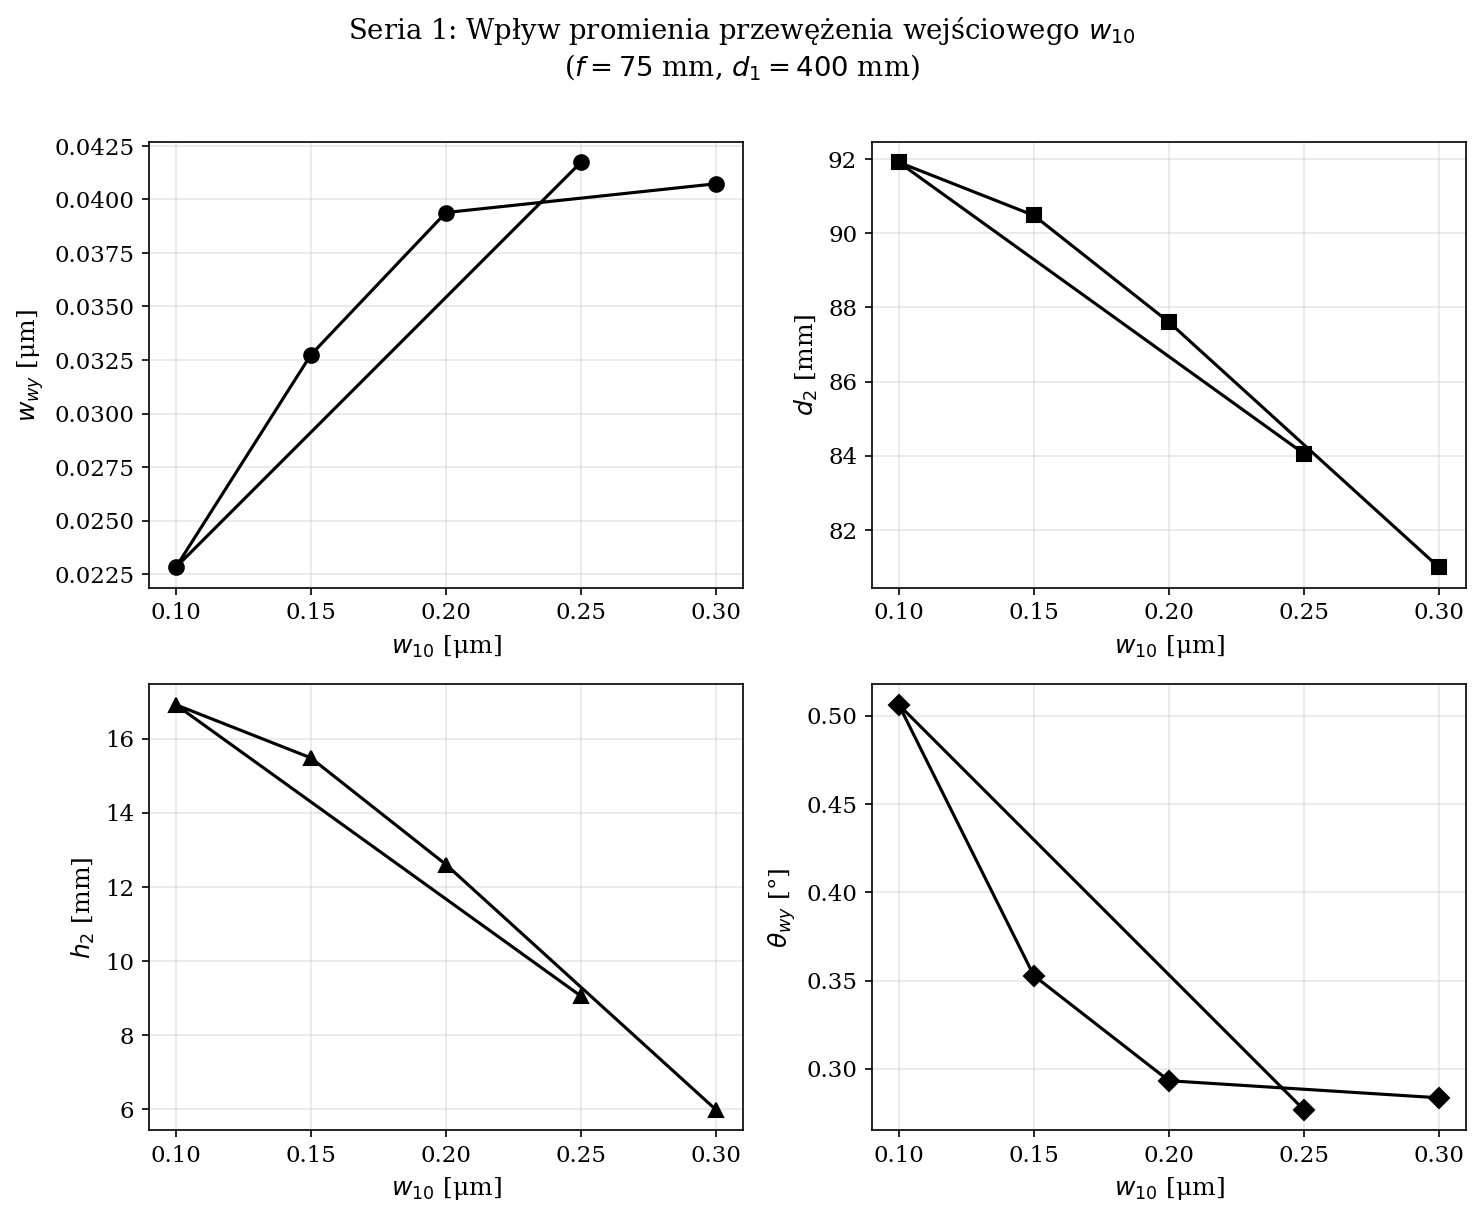
\includegraphics[width=\textwidth]{wykres_seria_w10.png}
\caption{Wpływ $w_{10}$ na parametry wiązki wyjściowej ($f=75$ mm, $d_1=400$ mm).}
\end{figure}

\begin{figure}[H]
\centering
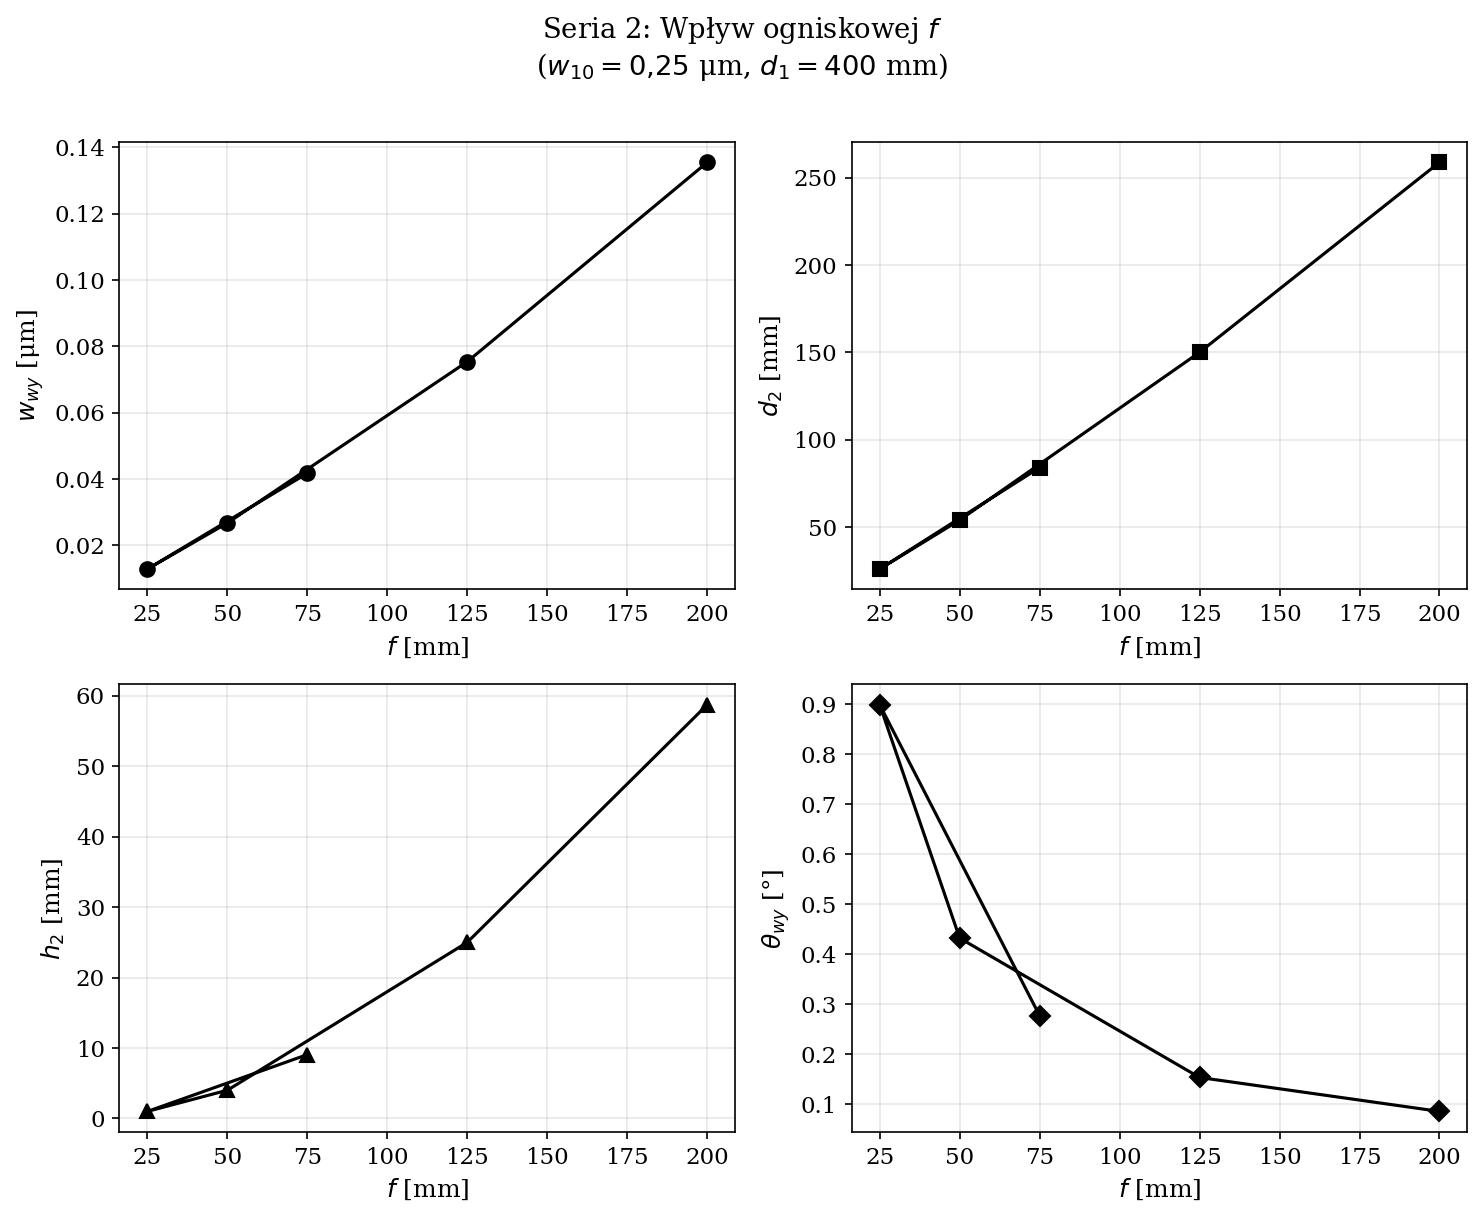
\includegraphics[width=\textwidth]{wykres_seria_f.png}
\caption{Wpływ $f$ na parametry wiązki wyjściowej ($w_{10}=0{,}25$ \si{\mu m}, $d_1=400$ mm).}
\end{figure}

\begin{figure}[H]
\centering
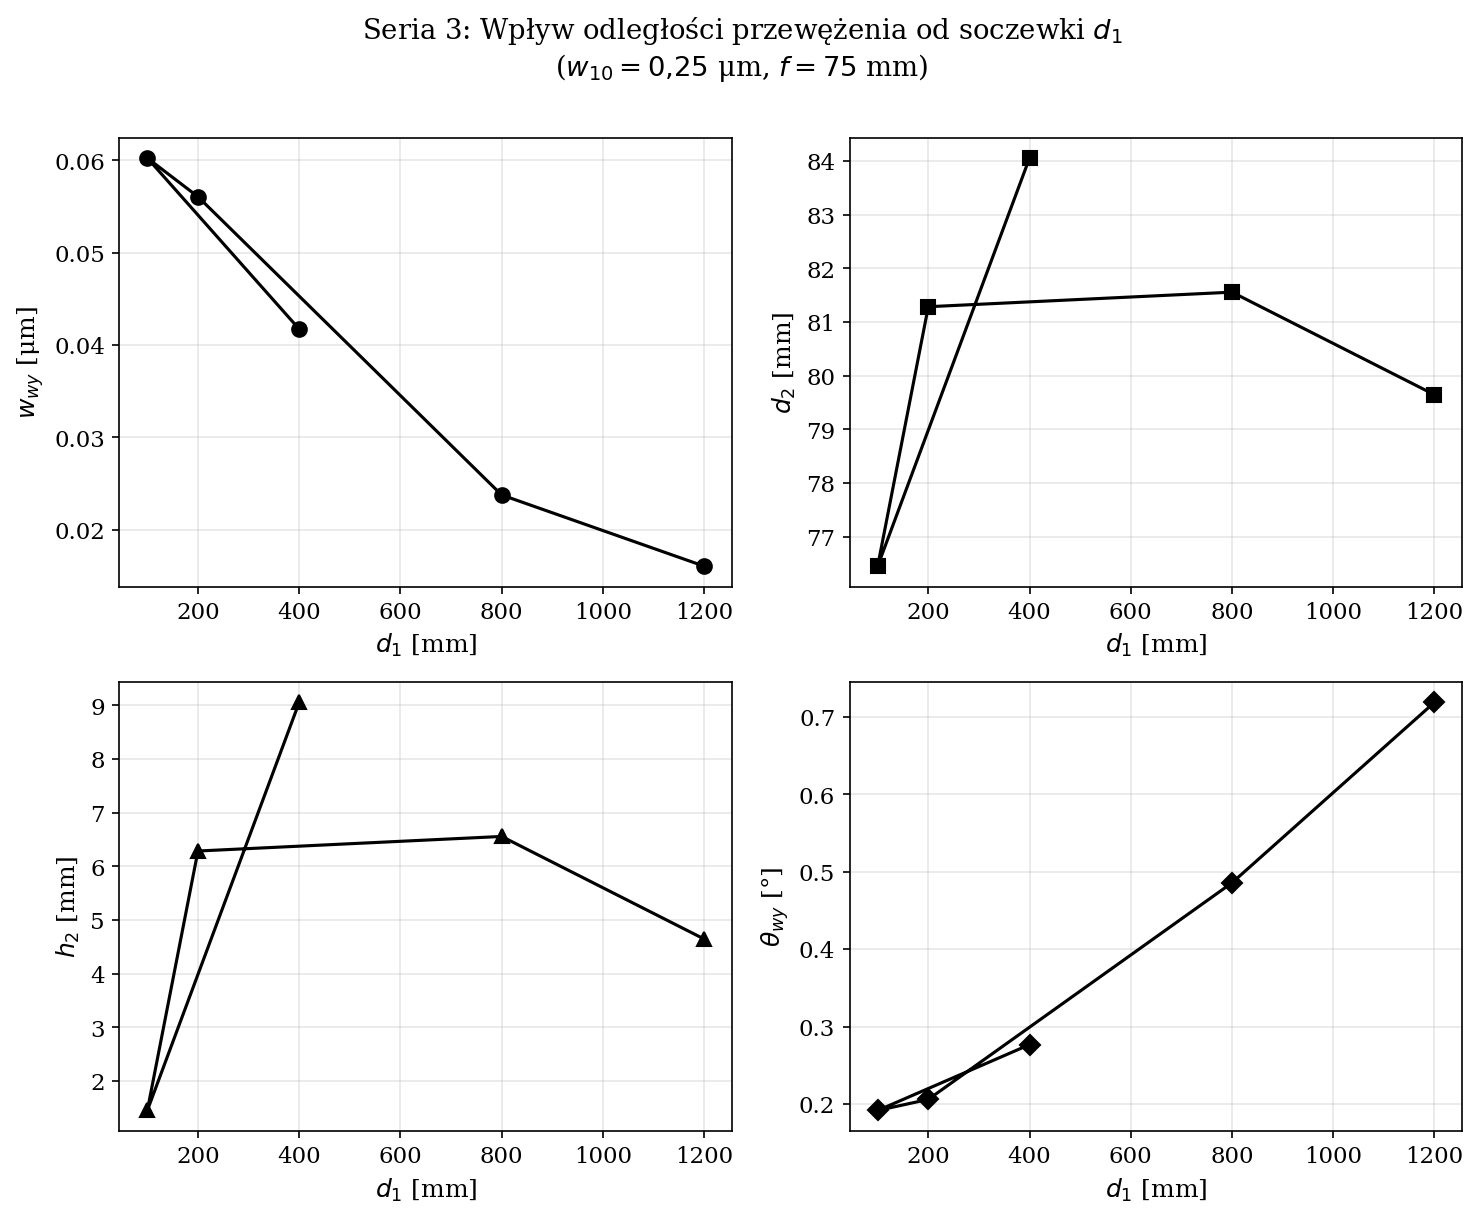
\includegraphics[width=\textwidth]{wykres_seria_d1.png}
\caption{Wpływ $d_1$ na parametry wiązki wyjściowej ($w_{10}=0{,}25$ \si{\mu m}, $f=75$ mm).}
\end{figure}

\section{Wykresy z symulacji}

Poniżej zamieszczono wykresy profilu wiązki przed i za soczewką, wygenerowane w Pythonie na podstawie kodu MATLAB-owego \texttt{Gauss\_soczewka\_skupiajaca.m}. Wykresy przedstawiają obwiednię $w(z)$ dla obu stron soczewki, oś optyczną, położenie soczewki oraz ogniska.

\begin{figure}[H]
\centering
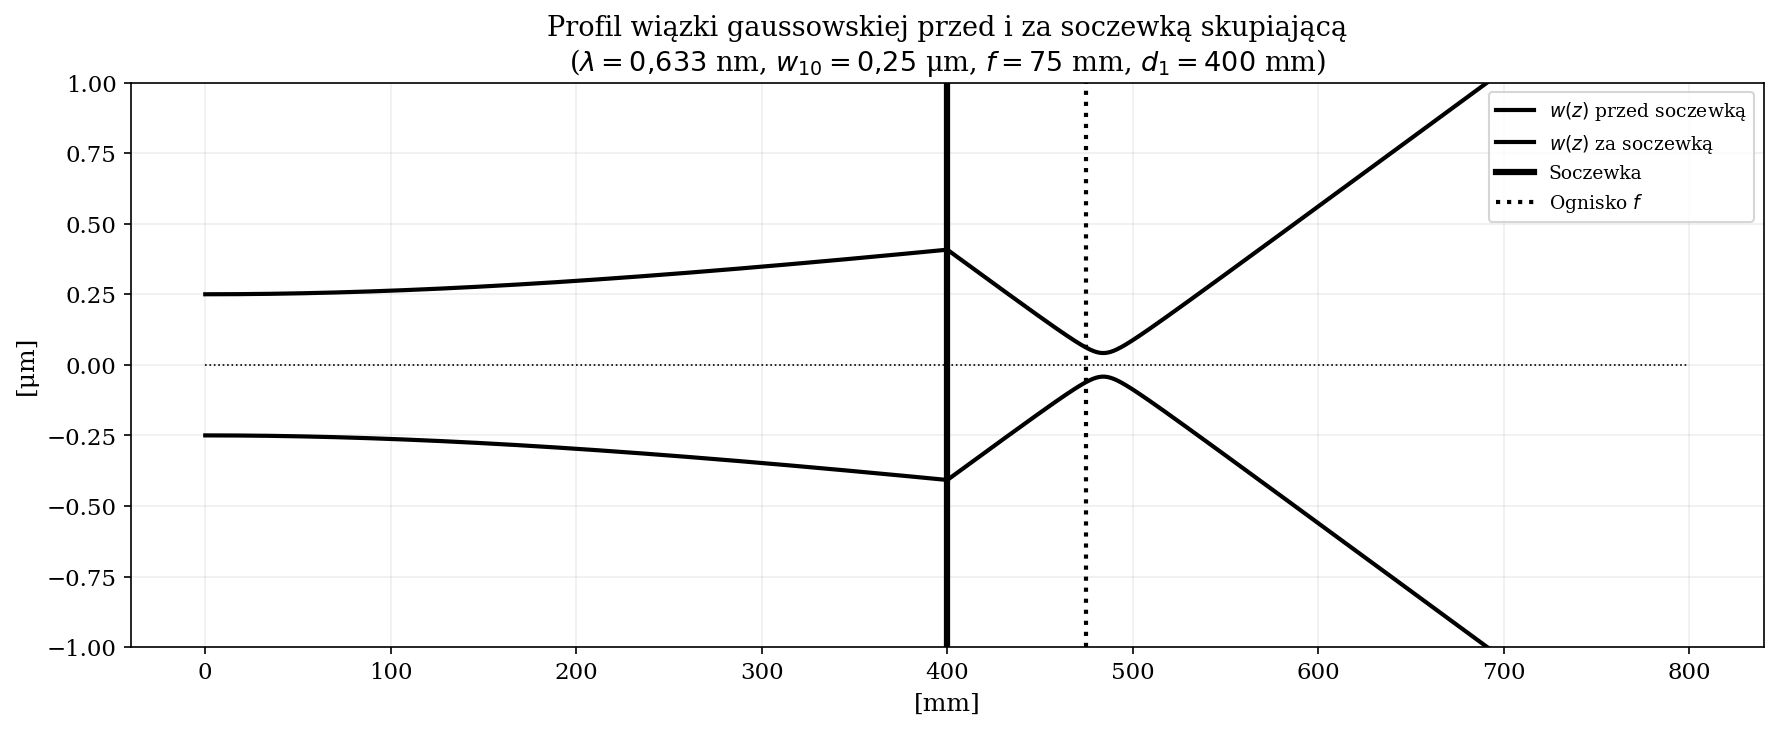
\includegraphics[width=0.95\textwidth]{profil_wiazki_domyslny.png}
\caption{Profil wiązki gaussowskiej dla wartości domyślnych: $\lambda = \SI{0,633e-3}{mm}$, $w_{10} = \SI{0,25}{\mu m}$, $f = \SI{75}{mm}$, $d_1 = \SI{400}{mm}$.}
\end{figure}

\begin{figure}[H]
\centering
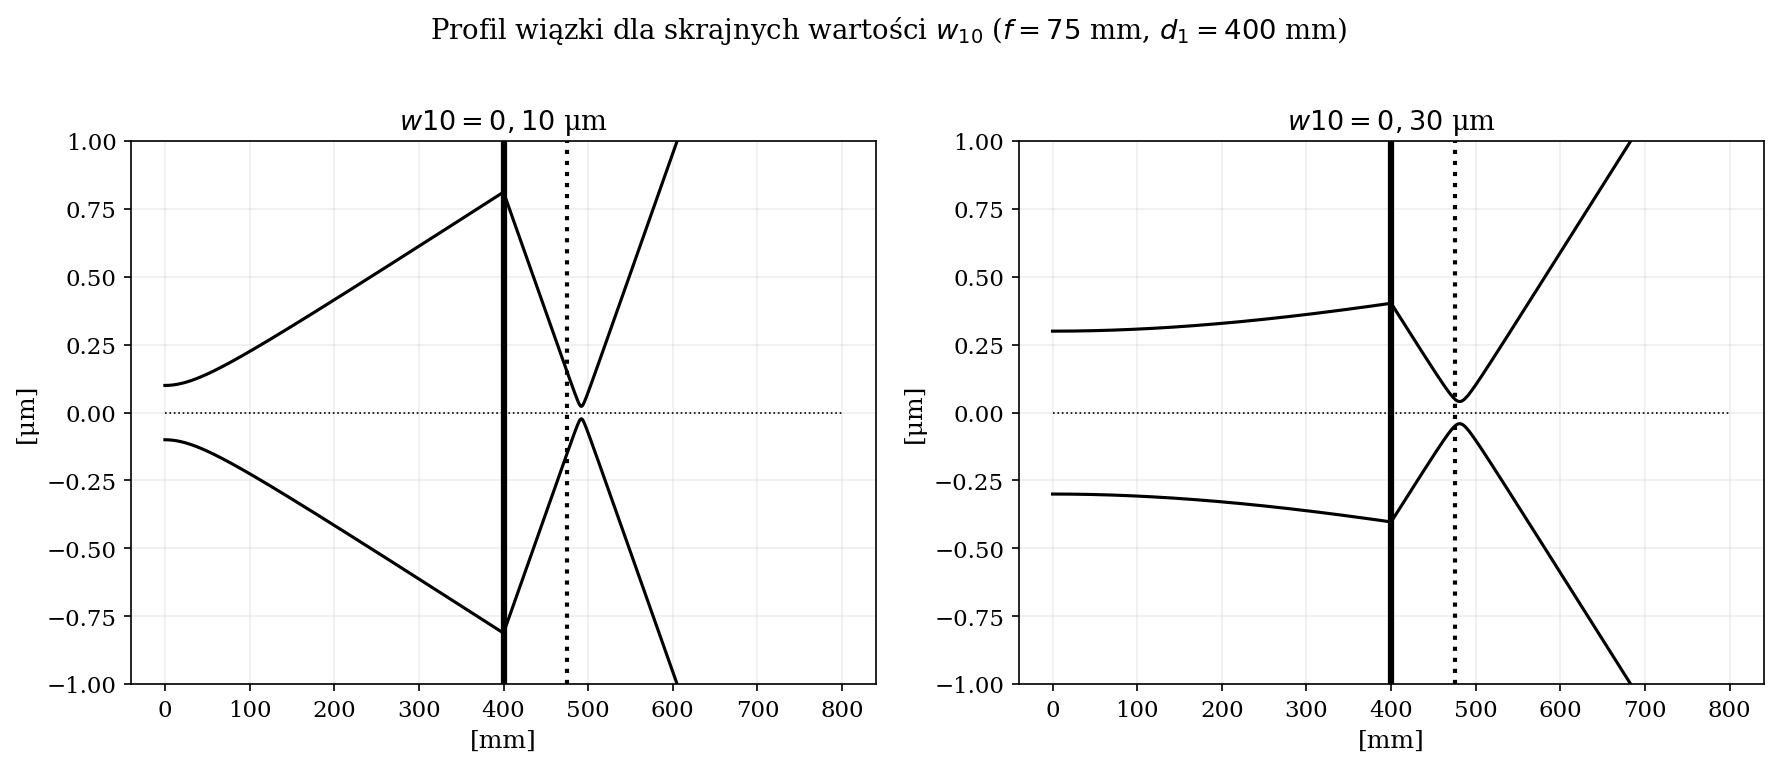
\includegraphics[width=0.95\textwidth]{profil_w10_skrajne.png}
\caption{Porównanie profili wiązki dla skrajnych wartości $w_{10}$ (0,10 i \SI{0,30}{\mu m}).}
\end{figure}

\begin{figure}[H]
\centering
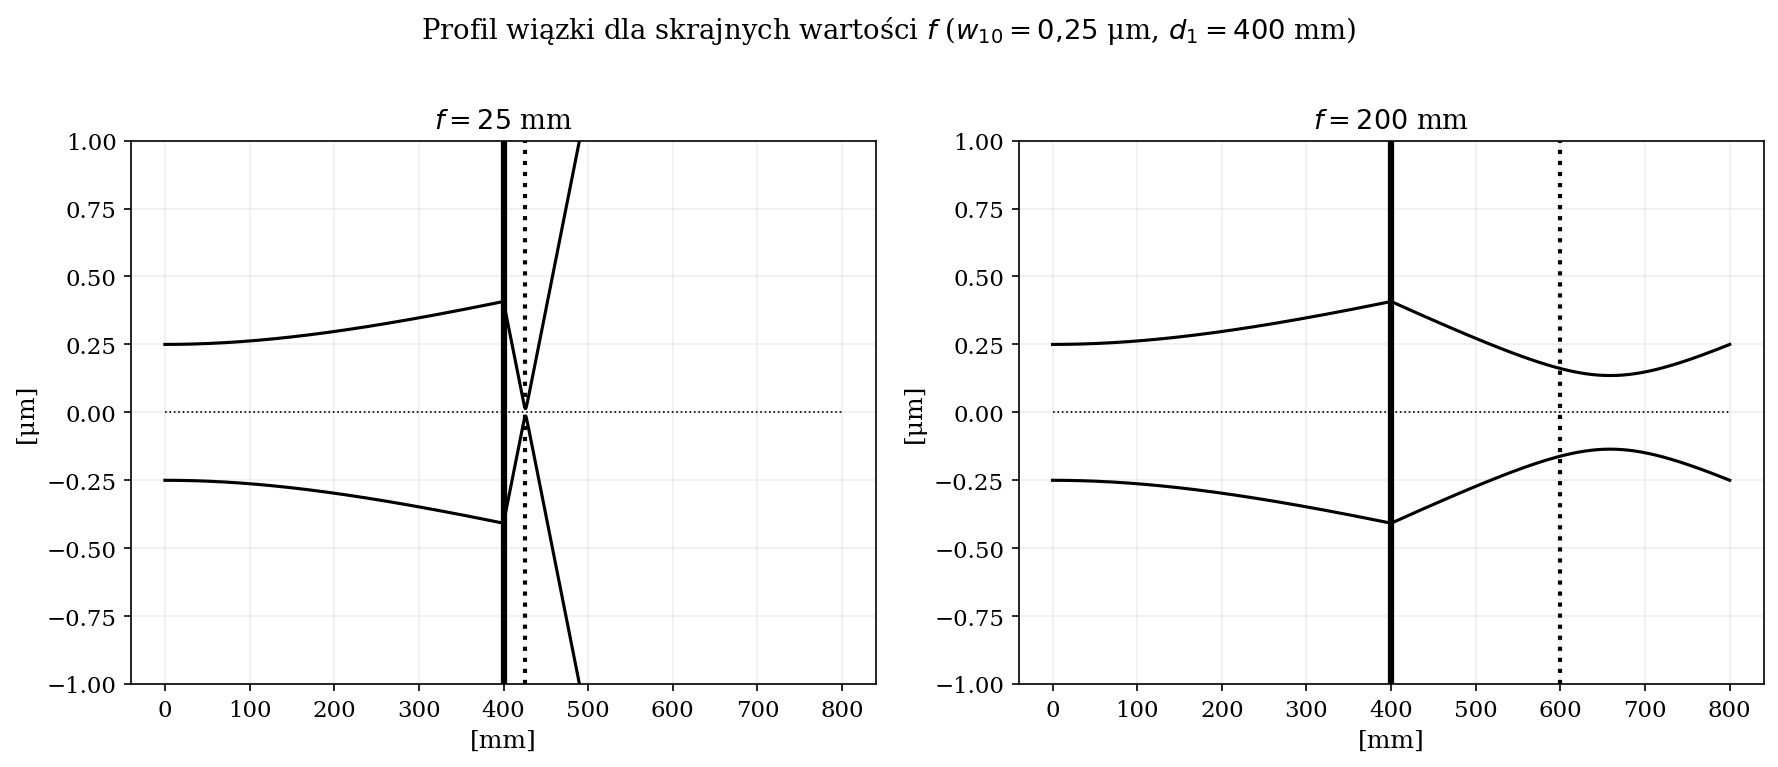
\includegraphics[width=0.95\textwidth]{profil_f_skrajne.png}
\caption{Porównanie profili wiązki dla skrajnych wartości $f$ (25 i \SI{200}{mm}).}
\end{figure}

\section{Wnioski}

\begin{enumerate}
\item \textbf{Wpływ $w_{10}$ (promienia przewężenia wejściowego):}
  Zwiększenie $w_{10}$ powoduje wzrost $w_{wy}$, co wynika z~bezpośredniej zależności we wzorze (3). Jednocześnie rośnie $z_{R1}$ (zasięg Rayleigha), przez co wiązka pada na soczewkę z mniejszą rozbieżnością kątową. Większe $w_{10}$ daje mniejsze $\theta_{wy}$, co jest zgodne z niezmiennikiem $w_{wy}\theta_{wy} = \lambda/\pi$. Dla $w_{10} = \SI{0,30}{\mu m}$ przewężenie wyjściowe jest największe, a kąt rozbieżności najmniejszy.

\item \textbf{Wpływ $f$ (ogniskowej):}
  Większa ogniskowa powoduje silniejszy wzrost $w_{wy}$ oraz $d_2$. Jest to zrozumiałe -- im dłuższa ogniskowa, tym słabsza moc optyczna soczewki ($P = 1/f$), więc wiązka jest słabiej skupiana. Dla $f = \SI{200}{mm}$ przewężenie $w_{wy}$ jest ponad 10 razy większe niż dla $f = \SI{25}{mm}$, a kąt rozbieżności odpowiednio mniejszy. $h_2 = d_2 - f$ rośnie z $f$, co oznacza że przewężenie wyjściowe oddala się od ogniska wraz ze wzrostem ogniskowej.

\item \textbf{Wpływ $d_1$ (odległości przewężenia od soczewki):}
  Zmiana $d_1$ wpływa na krzywiznę frontu falowego padającego na soczewkę. Dla małych $d_1$ (wiązka prawie równoległa przy soczewce) przewężenie wyjściowe znajduje się blisko ogniska ($h_2$ małe). Dla $d_1 = \SI{100}{mm}$ otrzymujemy największe $w_{wy}$ -- wiązka nie zdążyła się rozbiec przed soczewką. Przy większych $d_1$ rozbieżność wiązki przed soczewką rośnie, co skutkuje mniejszym $w_{wy}$ po przejściu.

\item \textbf{Kąt rozbieżności $\theta_{wy}$:}
  We wszystkich seriach zachowana jest odwrotna proporcjonalność między $w_{wy}$ a $\theta_{wy}$, zgodnie ze wzorem $\theta_{wy} = \lambda/(\pi w_{wy})$. Im silniej wiązka jest skupiona (mniejsze $w_{wy}$), tym szybciej się rozbiega po przewężeniu.

\item \textbf{Metoda ABCD:}
  Parametry wiązki po przejściu przez układ optyczny oblicza się poprzez transformację zespolonego parametru $q$ za pomocą macierzy ABCD elementu optycznego. Z~otrzymanego $q_{wy}$ odczytuje się część rzeczywistą (odległość do przewężenia) i urojoną (zasięg Rayleigha), a~następnie wyznacza $w_{wy}$ i $\theta_{wy}$. Dla soczewki cienkiej macierz ma prostą postać $[1,0; -1/f, 1]$, a równania redukują się do wzorów (3)--(6).

\item \textbf{Praktyczne znaczenie:}
  Możliwość przewidywania parametrów wiązki po przejściu przez soczewkę ma kluczowe znaczenie przy projektowaniu układów optycznych -- pozwala dobrać odpowiednią soczewkę do uzyskania żądanego przewężenia w~zadanej odległości, np. przy sprzęganiu wiązki laserowej ze światłowodem.
\end{enumerate}

\end{document}
